\documentclass{assignmeownt}
\usepackage{listings}
\usepackage{amsmath}
\usepackage{nccmath}
\usepackage{pdfpages}

\DeclareMathOperator*{\argmax}{arg\,max}
\DeclareMathOperator*{\argmin}{arg\,min}


\coursenumber{05124265}
\coursetitle{Reinforcement Learning}
\title{Exercise 3}
\author{Tal Grossman, 201512282 , Moshe Yelisevitch, 207423104}
\date{10/07/2024}


\begin{document}
\maketitle
\thispagestyle{firststyle}
\section{Theory}
for theory sections please see handwritten solution.

% hand written solution for question 1
\begin{figure}[h]
    \centering
    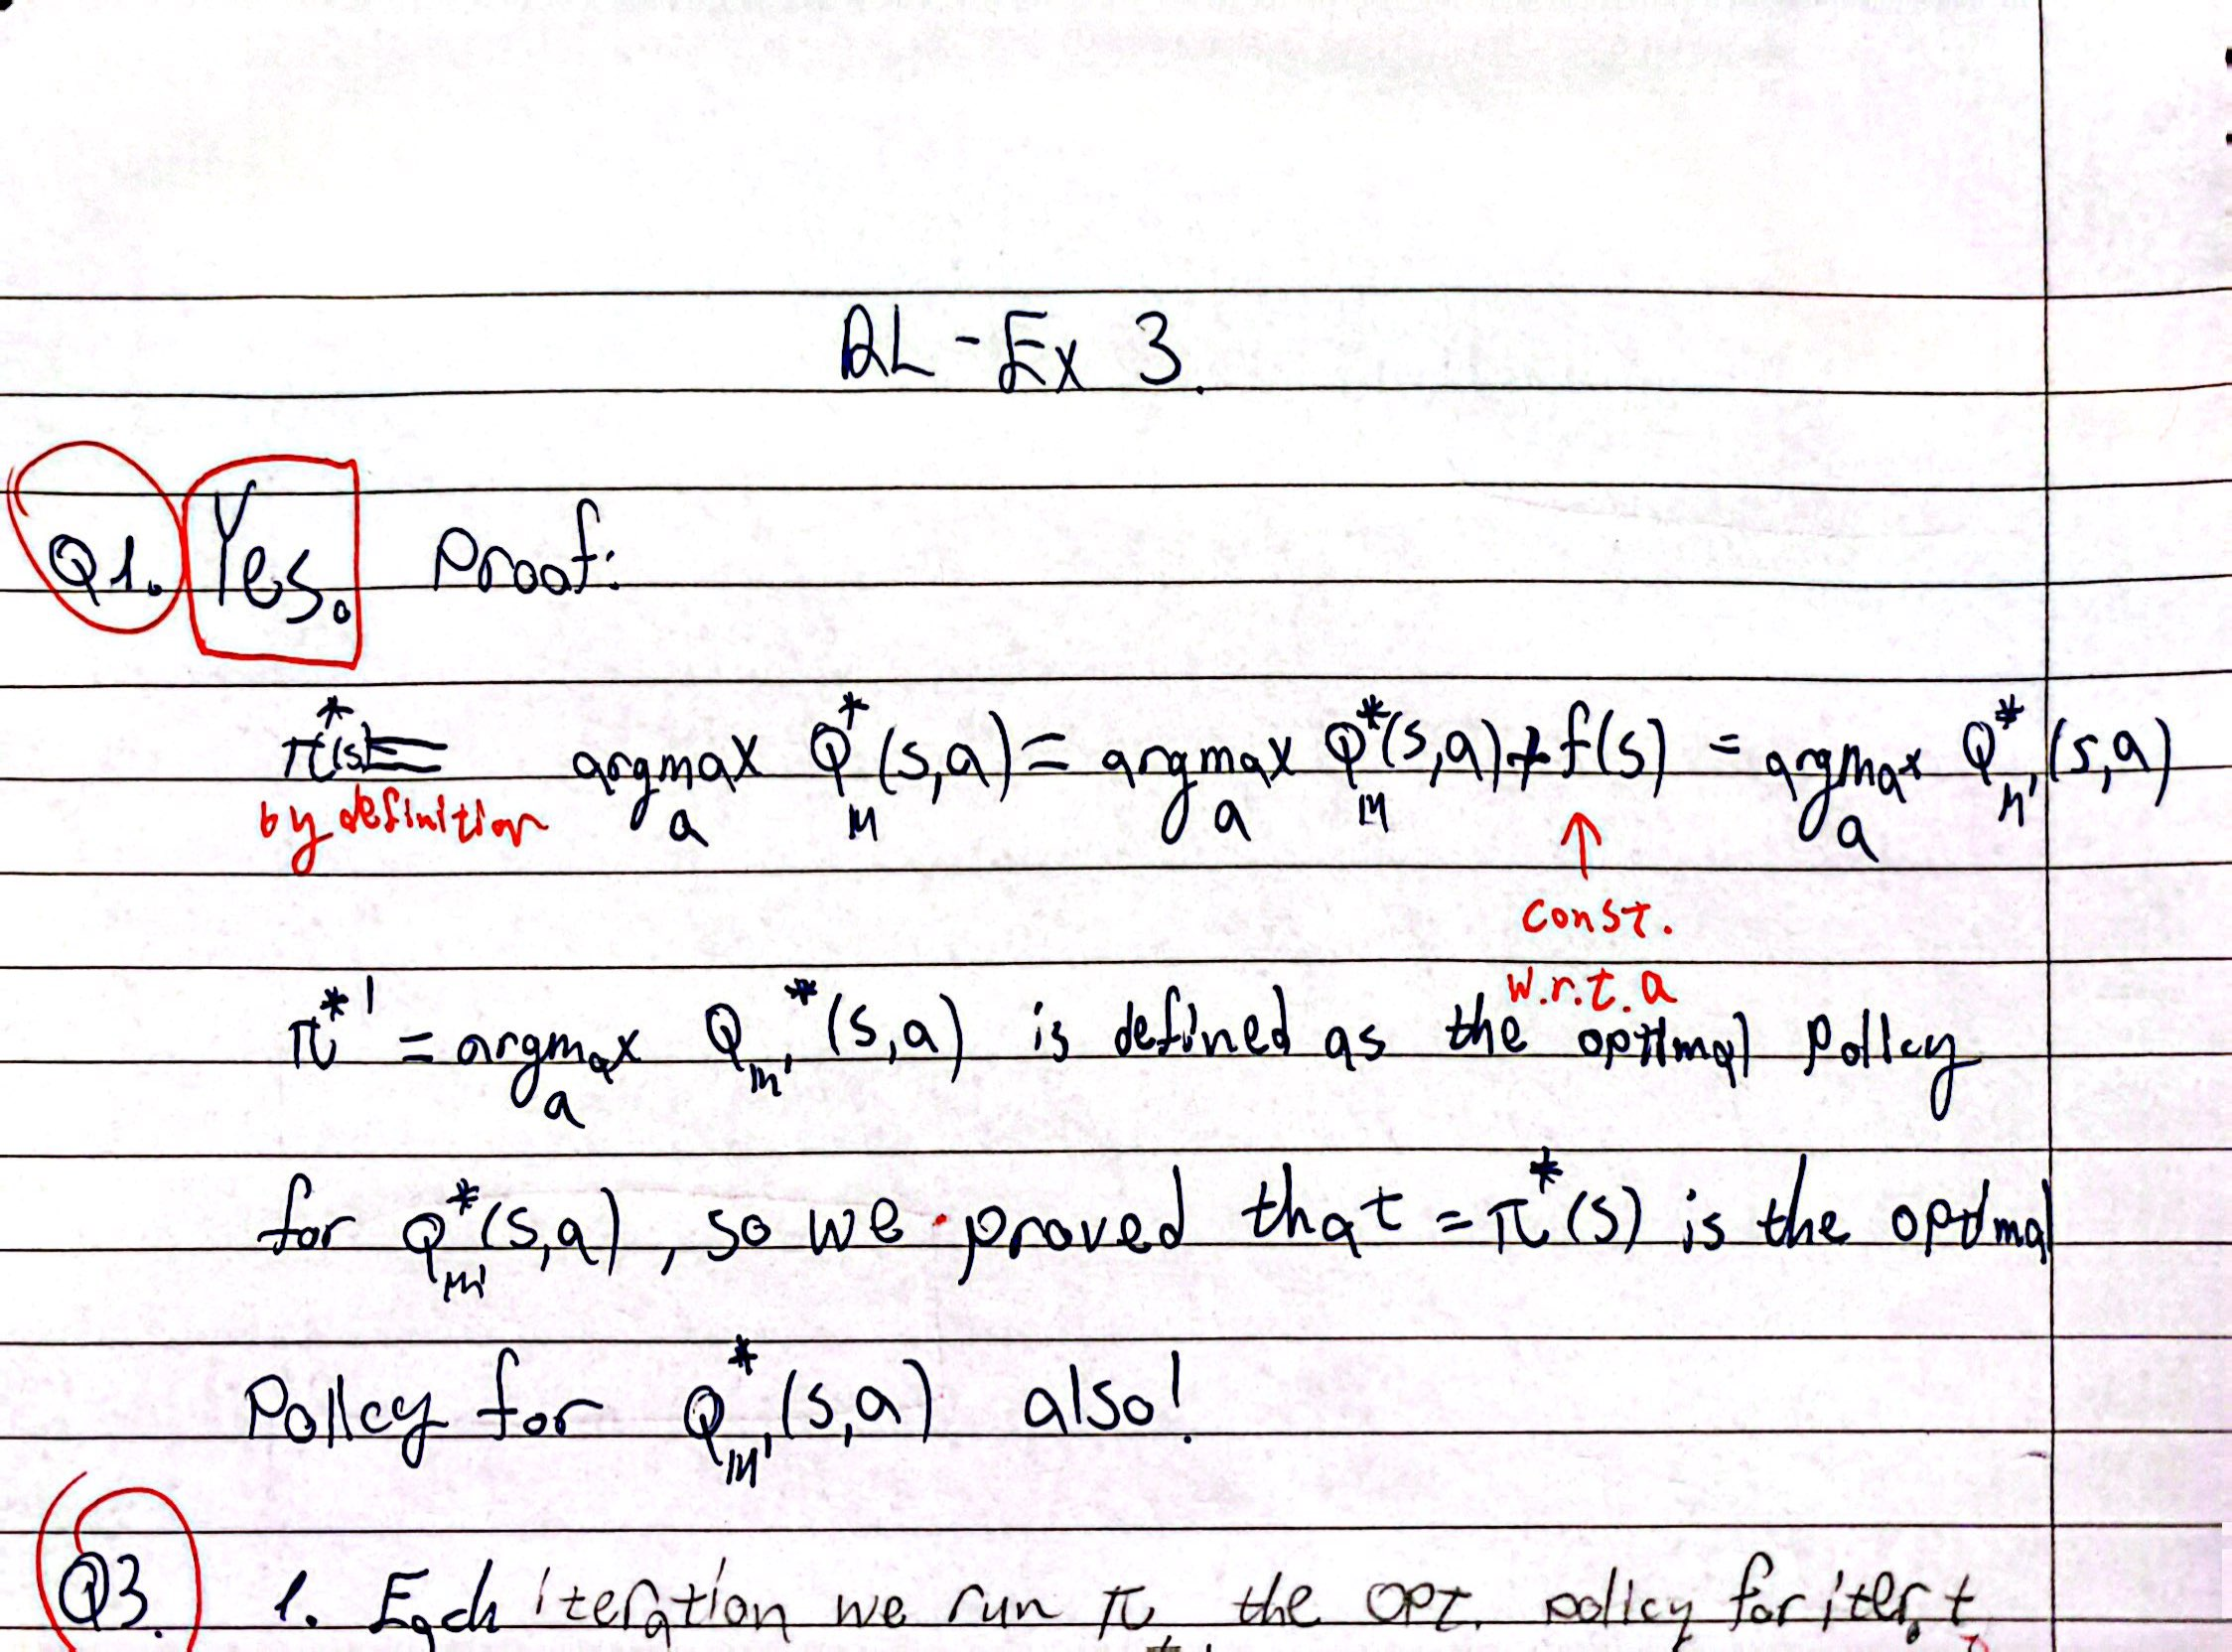
\includegraphics[width=\textwidth]{HW3_solution_Q1.jpg}
\end{figure}
% hand written solution for question 2 
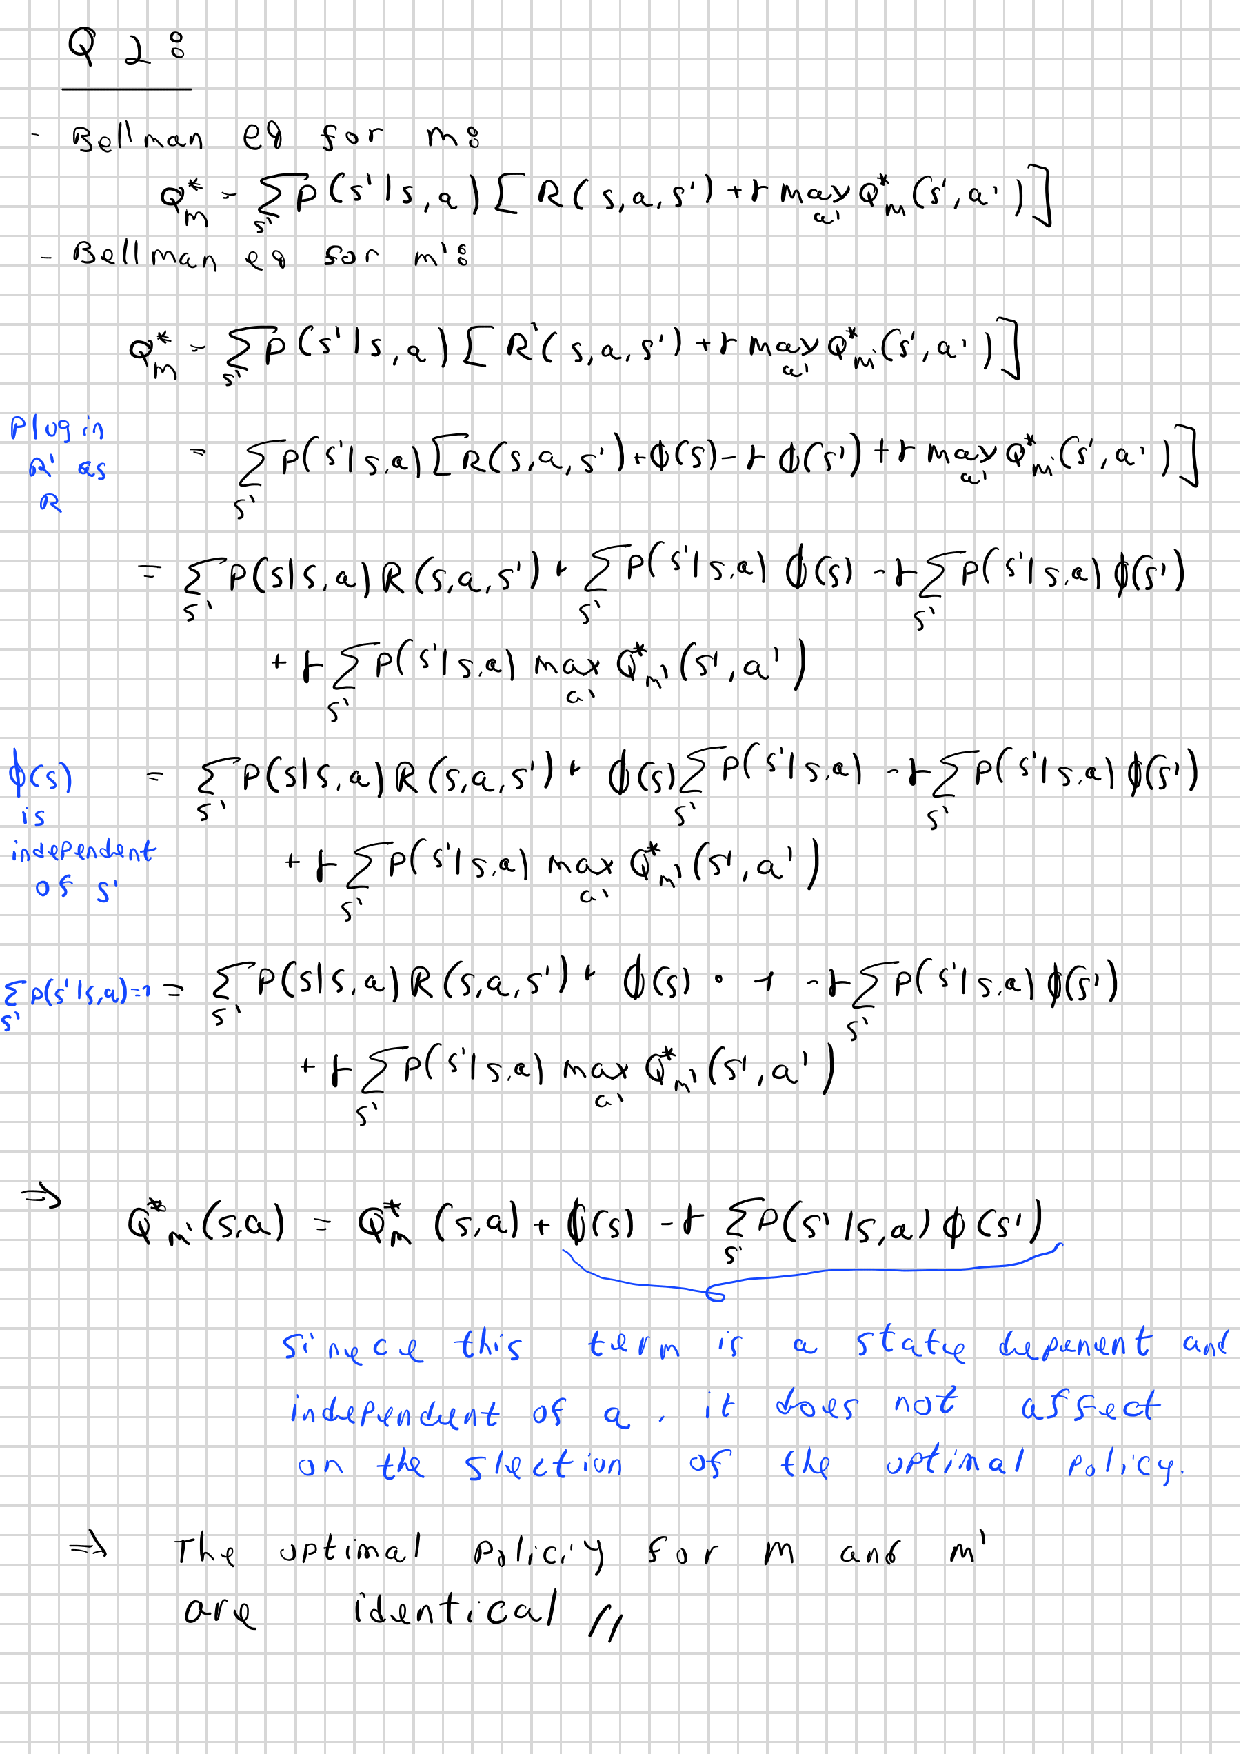
\includepdf[pages=1]{HW3 solution _sol2_4.pdf}
% hand written solution for question 3
\includepdf[pages=2-]{HW3_solution_Q3.pdf}
% hand written solution for question 4
\includepdf[pages=2-]{HW3 solution _sol2_4.pdf}

\newpage
\section{Programming}

\subsection{Question 1: Off-Policy Model-Based}
completed in python in the attached file \textbf{control.py}
\newline
In that specific run, it took 263 iterations to converge. The plot of the failure rate is as follows:
\begin{figure}[H]
    \centering
    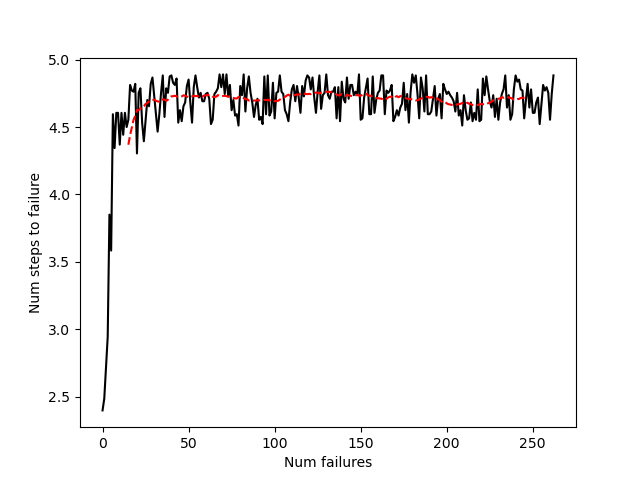
\includegraphics[width=0.7\textwidth]{ex1_263_failure_plot.png}
\end{figure}

\subsection{Question 2: Q-Learning}
\subsubsection{Item 1 - tabular\_Q.py}
The percentage of successful episodes is roughly \text{56.6\%} . The Q-table is as follows:
\begin{figure}[H]
\centering
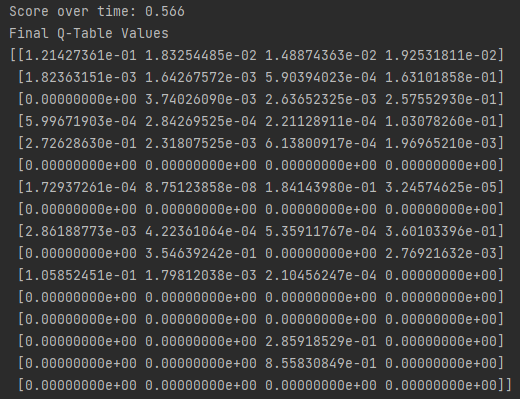
\includegraphics[width=0.6\textwidth]{Q_table_ex2_item1.png}
\end{figure}
\subsubsection{Item 2 - network\_Q.py}
The percentage of successful episodes is roughly \text{34.5\%}.
This result is worse than what we achieved with tabular Q-learning, probably due to the fact that the network is not
deep and complicated enough to capture the complexity of the environment. We believe that with a deeper network with
some activation functions, we could achieve better results.

\begin{figure}[H]
\centering
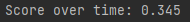
\includegraphics[width=0.4\textwidth]{score_ex2_item2.png}
\end{figure}

\end{document}
